%任何有关社会保险的选题均可,期末论文具体题目请自拟
%论文请用A4纸,字体宋体、正文字号五号,论文正文部分不超过15页。
\documentclass[a4paper,10.5pt]{ctexart}
\usepackage[style=gb7714-2015ay]{biblatex}
\usepackage{graphicx}
\usepackage{amsmath}
\usepackage{amssymb}
\usepackage{float}
\usepackage[hidelinks]{hyperref}
\providecommand{\keywords}[1]{\\\textbf{\textit{关键词:}}#1}
\addbibresource{reference.bib}
\title{个人养老金:全球视角与中国特色}
\author{董晨阳}
\date{\today}
\begin{document}
\maketitle
\thispagestyle{empty}
\begin{abstract}
    在这里写摘要。
    \keywords{关键词1,关键词2}
\end{abstract}
\setcounter{secnumdepth}{0}
\tableofcontents
\clearpage
\setcounter{page}{1}
\section{个人养老金的全球多样性}
发展个人养老金,是应对人口老龄化压力、完善养老体系的重要改革举措。经过长期论证,我国于2018年启动个人养老金制度建设,2022年加快部署:4月份国务院办公厅发布《关于推动个人养老金发展的意见》;6月份人社部、财政部、国家税务总局、银保监会、证监会联合印发《关于推动个人养老金发展的意见》宣传提纲,证监会发布《个人养老金投资公开募集证券投资基金业务管理暂行规定(征求意见稿)》,随着更多相关细则落地实施,个人养老金发展可能进入新阶段。
\begin{figure}[H]
    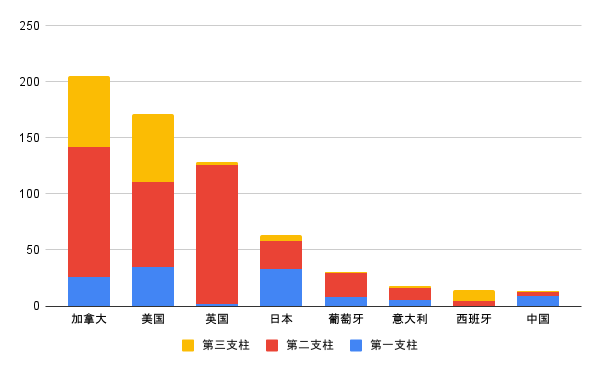
\includegraphics[width=\linewidth]{img/三支柱规模占GDP比重.png}
    \caption{养老储备规模与结构差异明显}
\end{figure}

由于海外发展个人养老金时间较久,可以为我国提供一定借鉴,当前大部分的养老金研究也以梳理国外案例为主,通过列举几个发达市场个人养老金的发展现状,然后套用到我国的养老金实践中。例如根据美国第一、二、三支柱养老金资产占GDP比重,预测中国未来的个人养老金规模。这种案例分析虽然可以提供一定信息,但是局限性也比较明显。由于各国的经济基础、人口结构、制度体系千差万别,不仅导致养老金总体规模差异明显,结构比重也大相径庭。美国个人养老金规模占GDP比重超过70\%,在养老储备中占比约40\%,而同属发达国家的日本,其个人养老金规模占GDP比重仅3.4\%,在养老储备中占比不足4\%。中国个人养老金的发展前景究竟应该对标美国还是日本?案例分析难以给出令人信服的答案。
\begin{figure}[H]
    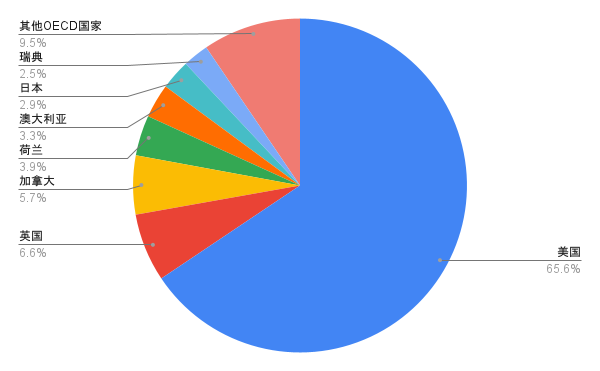
\includegraphics[width=\linewidth]{img/totalOECDpensionassets.png}
    \caption{养老金资产的全球分布极不均匀}
\end{figure}

分析个人养老金发展前景,确实需要参考海外市场经验,但是分析框架需要升级,不能停留在列举个别案例的层面,而应从全球养老金的多样化实践中寻找普遍规律,以此为基础推导我国乃至全球个人养老金的发展前景,并根据中国具体国情做出修正。本文根据过去20年中26个国家的个人养老金发展实践,从人口特征、经济基础、制度设计三个维度展开分析,研究中国与全球养老金的发展的共性与特性,提供一些分析与核算。
\section{文献综述}

\section{他山之石:海外养老金第三支柱发展经验}
\subsection{美国}
\subsection{日本}
\subsection{德国}

\section{个人养老金规模的影响因素}

\subsection{人口特征}
年龄结构变化首先促进养老金积累,然后可能会形成养老金减量压力。根据生命周期理论\cite{ando1963life},个体的收入水平随年龄不断变化,理性人会根据一生总收入安排消费与储蓄:在年轻阶段,收入大部分被消费掉甚至小于消费,往往形成负债,储蓄较少;中年阶段收入高于消费,偿还年轻时的负债,并为退休阶段准备养老资金,储蓄积累较快;进入老年阶段,消费下降但收入下降更多,需要使用中年阶段积累的养老资金,储蓄增长放缓甚至减少。因此随着年龄增长,储蓄水平先上升后下降。使用老年抚养比把全球主要国家分为四组,观察2010-2020年的个人养老金积累速度,可以发现随着老年抚养比提高,个人养老金积累速度开始放缓,但是在抚养比小于35\%时,个人养老金仍然可以实现较快积累;当抚养比小于20\%时,抚养比每提升1\%,个人养老金占GDP比重增加3.6\%;抚养比处于20\%-30\%之间时,养老金比重平均上升2.7\%;当抚养比在30\%-35\%之间,养老金比重增速降至1.2\%。只有当抚养比超过35\%,个人养老金占GDP比重才进入相对稳定状态。目前全球老年抚养比为14.8\%,联合国预测2075年左右升至35\%。在这个阶段,虽然消耗储蓄的75岁以上人口比重上升较快,但是55-74岁相对年轻的老年人口比重也在上升,而这个年龄阶段人口仍在积累储蓄,因此全球养老金在未来10年里可能仍会继续增长。与此同时,随着储蓄最多的中年人口比重下降,全球总体养老金积累速度可能开始放缓。由于不同国家老年化程度不同,养老金积累可能分化加剧,部分老龄化程度较深的国家甚至可能出现养老金减量的情况。
\begin{figure}[H]
    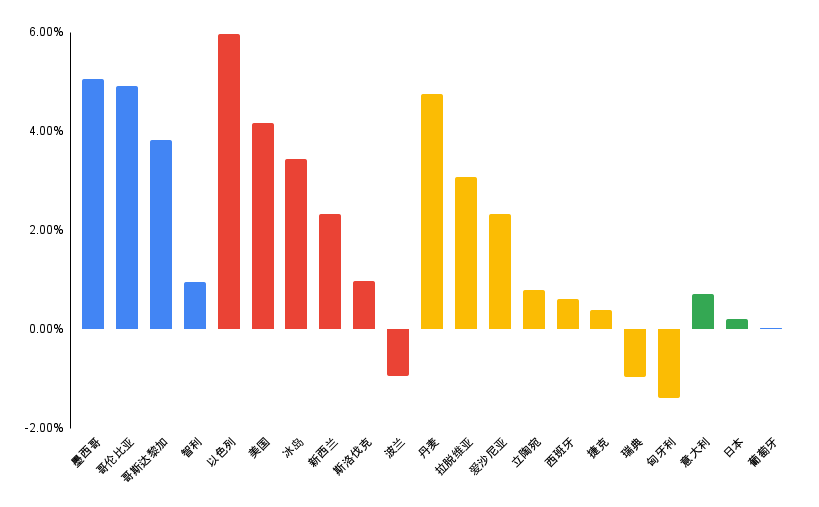
\includegraphics[width=\linewidth]{img/随着老年付养比提高,养老金积累增速开始下降.png}
    \caption{从左到右颜色对应老年抚养比0-20\%,20-30\%,30-35\%,35\%以上}
\end{figure}

预期寿命延长则促进养老金积累。在给定退休年龄的前提下,预期寿命延长意味着退休时间相较工作时间得到延长。根据生命周期理论,为平滑终身消费,居民需要在工作阶段积累更多的养老储蓄,用以退休后的消费支出,因此预期寿命和养老储蓄之间应该存在正相关性。从实证数据来看,伴随世界人口预期寿命的提升,全球储蓄占GDP的比重震荡上行,一定程度上反映了二者的正相关性;大量学术文献也得出了相一致的结论\cite{bloom2003longevity,de2009life},发现即使控制了居民收入、年龄结构等因素后,预期寿命的提升会显著提升居民储蓄率。由于个人养老金属于养老储蓄的一部分,因此预期寿命的延长会对个人养老金起到推动作用。
\begin{figure}[H]
    \begin{minipage}{0.48\linewidth}
        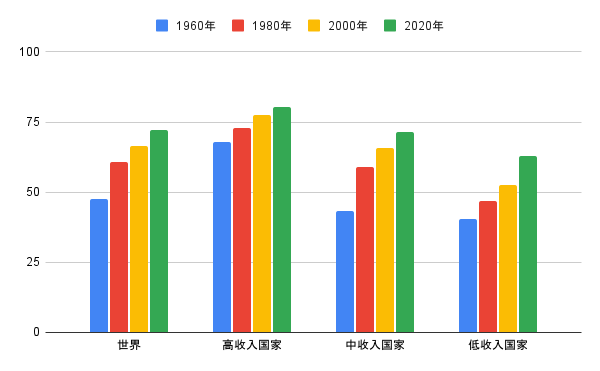
\includegraphics[width=\linewidth]{img/世界各国预期寿命普遍提升.png}
        \caption{世界各国预期寿命普遍提升}
    \end{minipage}
    \begin{minipage}{0.48\linewidth}
        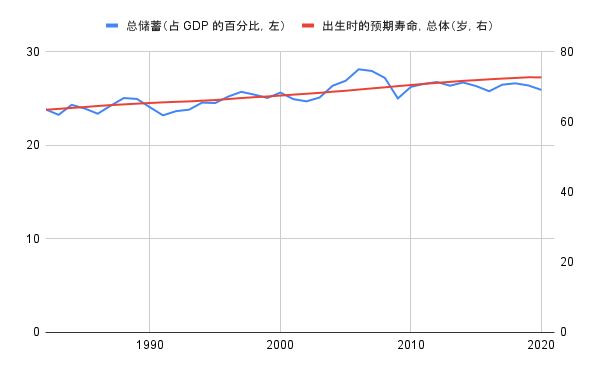
\includegraphics[width=\linewidth]{img/人口预期寿命与储蓄占GDP比重同步上升.png}
        \caption{预期寿命与储蓄占GDP比重同步上升}
    \end{minipage}
\end{figure}

\subsection{经济基础}

个人养老金是一种储蓄,而收入水平是影响储蓄的关键因素。凯恩斯的《就业利息和货币通论》中提出了边际消费倾向递减的规律,即虽然居民消费会随着居民收入的增加而增加,但增加的收入中用于消费的比例会逐渐降低,相对应储蓄的比例会升高。边际消费倾向递减的规律决定了收入水平提高会提升储蓄率,相应个人养老金规模就可能越大,个人养老金规模与居民收入水平呈现出明显正相关。
\begin{figure}[H]
    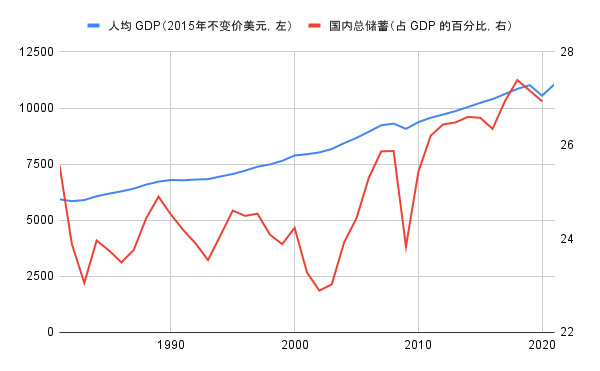
\includegraphics[width=\linewidth]{img/人均收入上升会提升储蓄率.png}
    \caption{人均收入上升会提升储蓄率}
\end{figure}

个人养老金也与居民资产配置结构相关。居民资产可分为实物资产和金融资产,个人养老金作为养老储蓄,也属于金融资产的范畴。与金融资产不同,以住房为代表的部分实物资产同时具备“实物”和“金融”双重属性,如果“金融”属性被放大,则会对个人养老金等其它金融资产形成挤压。部分国家的实证研究表明,高房价会对私人养老储蓄产生挤出效应。例如\citet{crawford2020impact}研究英国市场发现高房价会挤出私人养老金参与率,对于中等收入人群尤其明显,私人养老金发展规模与房地产相对价格呈现负相关。
\begin{figure}[H]
    \begin{minipage}{0.48\linewidth}
        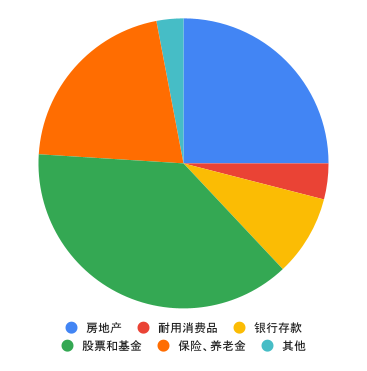
\includegraphics[width=\linewidth]{img/us.png}
        \caption{美国居民资产配置结构中房产占比仅约25\%}
    \end{minipage}
    \begin{minipage}{0.48\linewidth}
        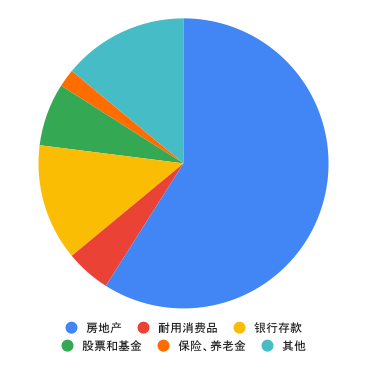
\includegraphics[width=\linewidth]{img/cn.png}
        \caption{中国居民资产配置结构中房产占比接近60\%}
    \end{minipage}
\end{figure}

我国居民资产配置失衡不仅体现在以房产为代表的实物资产占比过高,在金融资产内部也存在配置失衡,后者主要受我国金融发展水平影响。从广义角度讲,金融作为资金供给-需求的中间桥梁,其发展水平决定了储蓄-投资的转换效率,影响收入分配和资产配置格局,进而左右个人养老金的发展。金融发展受制度性因素影响较大,尤其是在发展中国家中,普遍存在金融抑制现象。金融抑制的概念最早由\citet{fishkin1973moral}提出,指政府干预金融市场而阻碍金融发展的现象,主要表现为利率(上限)管制、流动性比率限制、高存款准备金率、资本管制、金融市场准入门槛、信贷额度或分配限制、银行国有化等。金融抑制会阻碍个人养老金的发展,主要体现在需求和供给两个方面:从需求端,在金融抑制的环境中,由于存款利率被严重压低,实际上形成了一种居民补贴企业的效果,同时诱导企业选择低成本的资本密集型技术,以资本替代劳动,导致居民收入在国民收入分配中所占份额下降\cite{陈斌开2012金融抑制},对养老储蓄形成挤出;在供给端,由于高度依赖银行体系并存在资本账户管制,金融资产形式单一,直接融资市场发展不完备,养老产品供给缺乏,居民养老投资选择范围有限。

投资收益率提高,可以促进个人养老金积累。从资产增值的角度,投资收益率的提高会加速个人养老金所积累资产的增值,与此同时根据生命周期理论,高收益率可能会吸引个人投资者减少当期消费、增加储蓄,并提升个人养老金相较其它个人储蓄(如定期存款)的吸引力,将其他个人储蓄转化为个人养老金。
\begin{figure}[H]
    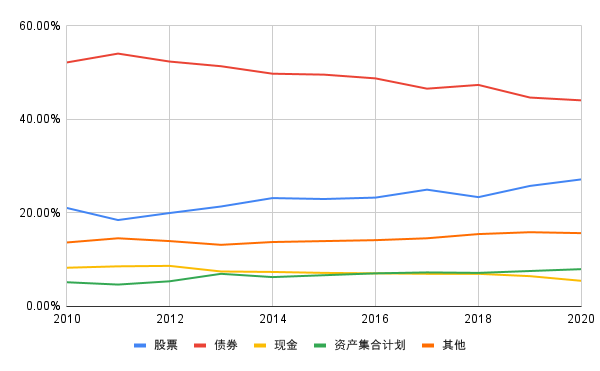
\includegraphics[width=\linewidth]{img/OECD国家私人养老金资产配置中股票占比不断上升.png}
    \caption{OECD国家私人养老金资产配置中股票占比不断上升}
\end{figure}

\subsection{制度设计}
第一二支柱的发展状况,会影响第三支柱个人养老金发展。由于公共养老金大多采用现收现付制,养老金资产存量未必准确反映养老金实际经济影响,个人养老金发展规模与公共养老金的支出规模存在较强的负相关关系,反映二者的替代效应。如果公共养老金支出规模较大,势必需要政府财政或居民缴费的支撑,在此背景下居民当期可支配收入减少,降低了于私人储蓄。与此同时,公共养老金支出较高,一般替代率水平也比较高,已经可以满足大部分居民的养老需求,积累私人养老金的必要性下降。

个人养老金和企业养老金同属于私人养老金,总体来看二者的发展具有正相关性,主要由于二者属性相似,均为基金积累制,且税收优惠制度相似。但与此同时,二者也具有竞争性:企业养老金相较个人养老金更具吸引力:企业年金一般会由企业或政府配资,且部分国家企业养老金具有强制性或半强制性,或引入自动加入机制,而个人养老金一般为自愿型。促进个人养老金发展的关键机制设计在于转化机制。如果没有相互转化机制,由于企业年金更具优势,往往个人养老金发展相对缓慢;而如果存在相互转化机制,个人养老金一般能获得更好发展。以美国为代表,企业年金发展会推动个人养老金发展。事实上美国家庭向个人养老金中缴存的比例较低,其资金来源主要以401(k)等企业或其它养老计划的转存流入为主,占比高达90\%以上。

最后,税优制度也对个人养老金有一定的促进作用。世界各国普遍采用税收激励的方式以支持个人养老金发展,这也是个人养老金与普通银行存款等其它投资储蓄账户的主要区别之一。目前世界上主流的免税激励模式是EET型,即在缴费和资本利得阶段享受税收优惠,在提取阶段需要偿还税收优惠。通过简单计算即可发现,EET模式相较正常储蓄账户具有显著的税收激励效果。其中,资本利得税在EET免税激励模式中发挥了重要作用,普通储蓄账户的资本利得税越高,养老金账户在EET模式下所享受的税收优惠程度就越大,进而促进个人养老金的发展

\section{中国特色}
\subsection{个人养老金政策与产品现状}
政策设计上,自2018年启动建立养老保险第三支柱工作以来,我国个人养老金账户政策逐步细化。对比国外相关规定,当前我国个人养老金政策的主要特征为
\begin{enumerate}
    \item 参与主体覆盖面广,参与自由。我国三支柱个人账户允许在中国境内参加一支柱养老保险的全体劳动者参与,第一支柱养老保险当前已覆盖约10亿人口。相比之下,第二支柱参保前提为供职企业设立企业年金,故三支柱养老覆盖面更广,参与更加自由。这一制度设计与美国IRA账户思路基本一致。值得一提的是,该制度的建立对于广大无法参加第二支柱养老体系的灵活就业人员意义重大,有望成为当前社会保障制度的重要补充。
    \item 出资与主体:自愿开立,个人出资,个人管理。第三支柱养老体系完全由个人出资,采用完全积累制。不同于第一支柱与第二支柱的统一专户委托管理,第三支柱资金由个人作为投资决策主体。我国试点政策缴纳额度上限最高为12000元,占当年平均工资百分比16.2\%,高于IRA的13.1\%,但低于DC计划38.4\%,符合三支柱特征。
    \item 账户投资范围:投资自由度相对前两支柱较高。个人自主选择购买符合规定的储蓄存款、理财产品、商业养老保险、公募基金等金融产品(统称个人养老金产品)。考虑到投资者教育水平等因素,我国相较于美国IRA账户投资自由度更低。
    \item 账户开立:养老资金账户仅能在商业银行开立,其他符合规定的金融产品销售机构可代销养老主题金融产品,商业银行把握资金入口,而美国无相关限制。
    \item 资金提取:有待进一步细化。参加人达到领取基本养老金年龄、完全丧失劳动能力、出国(境)定居等经信息平台核验领取条件后,可以按月、分次或者一次性领取个人养老金,领取方式一经确定不得更改,暂未规定强制提取年龄,也未明确提前支取的惩罚性条款。
\end{enumerate}

截至2022年11月25日,个人养老金产品主要有:
\begin{enumerate}
    \item 个人养老储蓄:首批23家商业银行发行的储蓄存款(包括4家国有大行发行的特定养老储蓄)
    \item 个人养老金理财产品:包括养老理财产品及其他理财产品,已纳入养老理财试点的11家理财公司可以参与,需要将拟参与个人养老金运行的理财产品报送银保监会。
    \item 个人养老金保险产品:包括年金保险、两全保险,以及银保监会认定的其他产品。目前包括6家机构的7只专属商业养老保险产品。
    \item 个人养老金公募基金:试行阶段,优先纳入养老目标基金,后续适时逐步纳入其他基金。目前包括40家公募机构的129只养老目标基金。
\end{enumerate}

\subsection{三支柱养老布局展望}
综合海外养老资管行业发展特征与我国发展形势,三支柱养老发展空间广阔。

居民收入持续提升有助于提升潜在账户持有率。美国账户持有比例与家庭收入正相关。据ICI统计,家庭年收入在2.5万美元及以下的美国家庭IRA持有率仅9\%;而年收入20万美元及以上家庭IRA持有率则高达65\%,且持有率随家庭年收入提升稳定正增。自2012年至2020年,我国城镇职工平均年薪已自4.0万元升至7.4万元,同期平均个人可支配收入从1.7万元提升至3.2万元,均有显著提升。结合海外经验,三支柱养老账户建设经济基础已有显著改善。
\begin{figure}[H]
    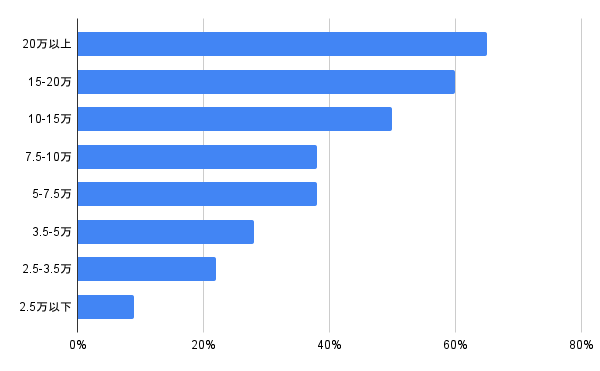
\includegraphics[width=\linewidth]{img/美国家庭持有IRA的比例与收入显著正相关.png}
    \caption{美国家庭持有IRA的比例与收入显著正相关}
\end{figure}

人口老龄化深化演进唤醒居民养老意识,提升账户持有意愿。美国经验表明,IRA持有意愿在退休前与住户年龄显著正相关。ICI调查数据显示,在退休年龄(65岁)之前,美国家庭IRA持有率随家主年龄提升而提升。我国人口老龄化的深入演进有望进一步唤醒居民养老储蓄意识,提升三支柱账户持有意愿。
\begin{figure}[H]
    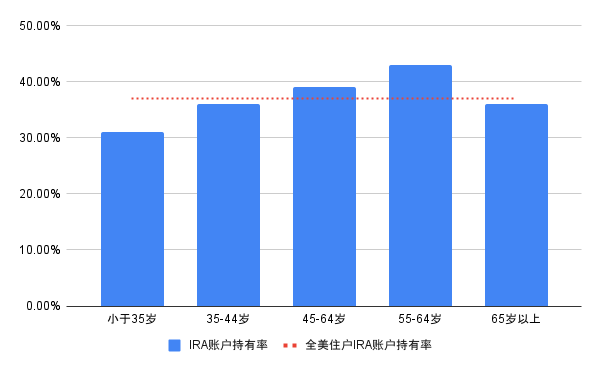
\includegraphics[width=\linewidth]{img/IRA账户持有率和全美住户IRA账户持有率.png}
    \caption{IRA账户持有意愿在退休前与住户年龄显著正相关}
\end{figure}

我国居民在养老金融上风险偏好低、对于银行系产品参与意愿更高。中国养老金融50人论坛对1.2万18岁以上、在城镇居住的人员进行调查。从风险承受上看,近五成调查对象可以阶段性承受10\%以内的亏损、近四成调查对象表示任何时候都不能出现亏损;从税优养老金融产品参与意愿来看,居民对于养老理财、养老储蓄和养老保险这类风险较低的产品参与意愿更高。
\begin{figure}[H]
    \begin{minipage}{0.48\linewidth}
        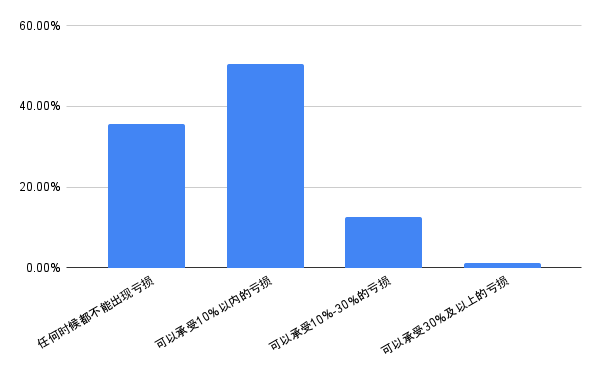
\includegraphics[width=\linewidth]{img/36调查对象无法承受任何亏损.png}
        \caption{36\%调查对象无法承受任何亏损}
    \end{minipage}
    \begin{minipage}{0.48\linewidth}
        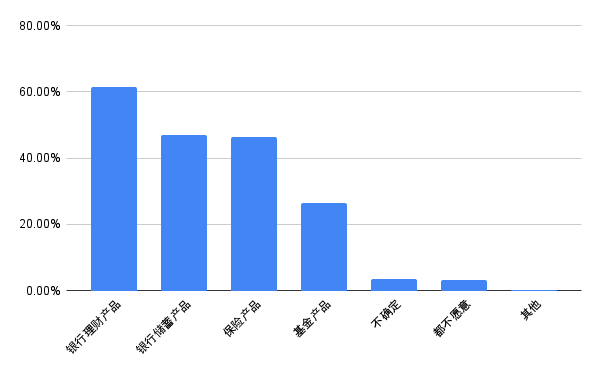
\includegraphics[width=\linewidth]{img/居民对于养老理财、养老储蓄及养老保险参与意愿更高.png}
        \caption{居民对于养老理财、养老储蓄及养老保险参与意愿更高}
    \end{minipage}
\end{figure}

\section{启示}
投资属性上看,商业养老保险具有保本属性、养老理财风险较低、养老基金风险和波动更高;服务属性上看,商业养老保险具备相对优势。养老金融产品包括投资属性和服务属性,从投资属性上看,商业养老保险采取保本+浮动收益,适合风险偏好较低的投资者。养老理财和养老基金均为非保本产品,其中养老理财整体投资期限更长、具有较高的业绩比较基准、产品费率低,同时具有风险保障机制以平滑波动,适合中低风险偏好的投资者;养老基金业绩比较基准以相对收益为主,费率更高,对应风险和收益更高,适合中风险及中高风险投资偏好人群。从服务属性上看,保险产品可附加康养等服务,未来将成为其差异化的竞争点。

短期而言,渠道端将自上而下影响产品配置。据《中国养老金融调查报告(2021)》调查,36\%调查对象选择养老金融产品途径为银行或其他金融机构,为选择养老金融产品的主要渠道。短期来看,渠道端将对居民资产配置影响较大。早期银行渠道较为强势,同时,居民风险偏好较低,相较于养老基金等风险较高的产品,储蓄和理财产品在风险程度上与我国养老人群更匹配;此外,养老理财凭借较高的业绩标准、低于其他养老金融产品的费率以及风险保障机制平滑基金波动等优势亦具备较强的吸引力。因此早期养老理财和养老储蓄或将具备较高份额。

长期而言,底层资产收益率将自下而上影响产品配置。伴随着市场利率下行,以及权益市场向好,养老基金将具备更高的收益和更强的吸引力。长期而言,银行产品的市场份额将部分分流至保险及基金产品,其中,保险产品以其保本+投资的属性将部分替代银行产品的保本功能,而基金产品以其相对较高的回报率将部分替代银行产品的收益功能。因此长期来看养老基金和养老保险市场份额将有所提升,养老储蓄和养老理财份额或将下滑。

\appendix
\nocite{*}
\printbibliography[heading=bibliography]
\end{document}
